\documentclass[tikz,border=4pt]{standalone}
\usepackage{amsmath,amssymb}
\usepackage{tikz}
\usetikzlibrary{arrows.meta,positioning,calc}

\definecolor{theoremgreen}{RGB}{219,234,226}
\definecolor{enginepurple}{RGB}{233,226,241}
\definecolor{foundationgray}{RGB}{235,235,235}
\definecolor{arrowpurple}{RGB}{100,71,153}
\definecolor{arrowgreen}{RGB}{43,125,79}

\tikzset{
  theorem/.style={
    draw=none, rounded corners=2pt, fill=theoremgreen,
    minimum height=1.55cm, text width=3.65cm, align=center,
    inner sep=5pt, font=\bfseries\small
  },
  engine/.style={
    draw=none, rounded corners=2pt, fill=enginepurple,
    minimum height=1.25cm, text width=4.4cm, align=center,
    inner sep=5pt, font=\small
  },
  foundation/.style={
    draw=none, rounded corners=2pt, fill=foundationgray,
    minimum height=1.5cm, text width=3.8cm, align=center,
    inner sep=5pt, font=\small
  },
  flow/.style={-{Stealth[length=2.2mm]}, line width=.8pt},
  engineflow/.style={-{Stealth[length=2.2mm]}, line width=.9pt, draw=arrowpurple},
  feed/.style={-{Stealth[length=2.2mm]}, line width=.8pt, draw=arrowgreen}
}

\begin{document}
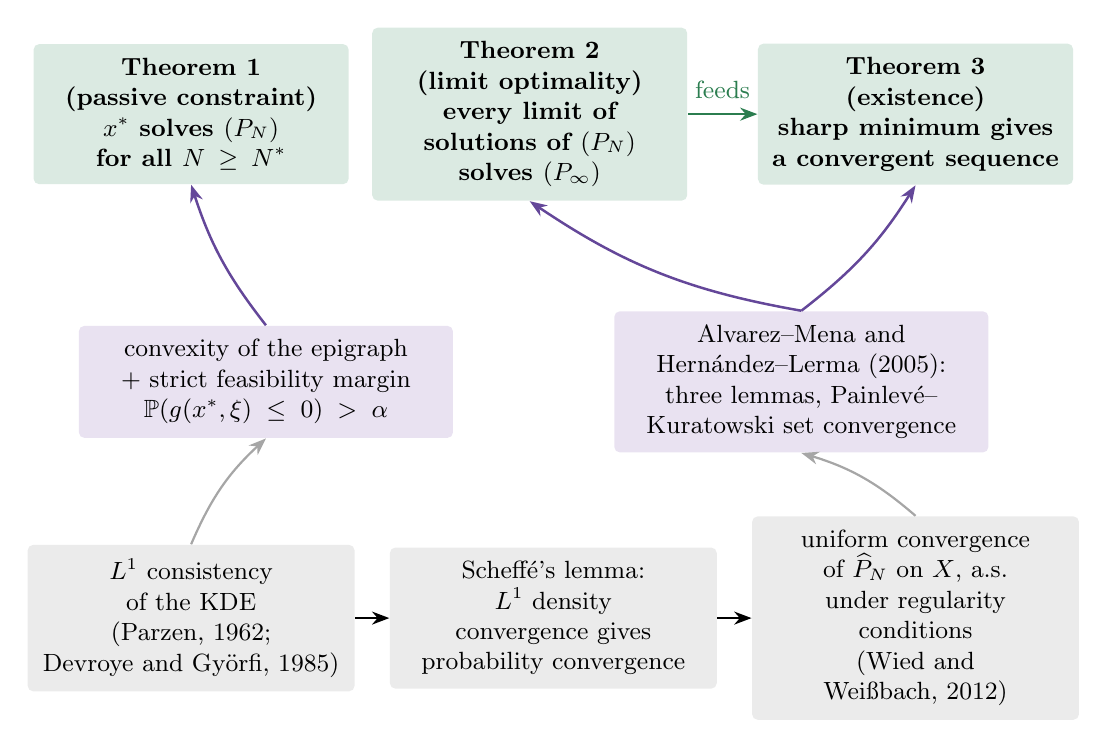
\begin{tikzpicture}[x=1cm,y=1cm]
  % Statistical foundation
  \node[foundation] (f1) at (2.2,0)
    {$L^1$ consistency of the KDE\\(Parzen, 1962;\\Devroye and Györfi, 1985)};
  \node[foundation] (f2) at (6.8,0)
    {Scheffé's lemma:\\$L^1$ density\\convergence gives\\probability convergence};
  \node[foundation] (f3) at (11.4,0)
    {uniform convergence\\of $\widehat P_N$ on $X$, a.s.\\
     under regularity\\conditions\\(Wied and Weißbach, 2012)};

  % Analytical engines
  \node[engine] (e1) at (3.15,3.0)
    {convexity of the epigraph\\+ strict feasibility margin\\
     $\mathbb P(g(x^*,\xi)\leq0)>\alpha$};
  \node[engine] (e2) at (9.95,3.0)
    {Alvarez--Mena and\\Hernández--Lerma (2005):\\
     three lemmas, Painlevé--\\Kuratowski set convergence};

  % Theorems
  \node[theorem] (t1) at (2.2,6.4)
    {Theorem 1\\(passive constraint)\\
     $x^*$ solves $(P_N)$\\for all $N\geq N^*$};
  \node[theorem] (t2) at (6.5,6.4)
    {Theorem 2\\(limit optimality)\\
     every limit of\\solutions of $(P_N)$\\solves $(P_\infty)$};
  \node[theorem] (t3) at (11.4,6.4)
    {Theorem 3\\(existence)\\
     sharp minimum gives\\a convergent sequence};

  % Horizontal statistical flow
  \draw[flow] (f1.east) -- (f2.west);
  \draw[flow] (f2.east) -- (f3.west);
  % Statistical foundation to analytical engines
  \draw[flow,draw=gray!70] (f1.north) to[bend left=12] (e1.south);
  \draw[flow,draw=gray!70] (f3.north) to[bend right=12] (e2.south);
  % Analytical engines to theorem statements
  \draw[engineflow] (e1.north) to[bend left=10] (t1.south);
  \draw[engineflow] (e2.north) to[bend left=12] (t2.south);
  \draw[engineflow] (e2.north) to[bend right=10] (t3.south);
  % Theorem 2 supplies the existence argument used by Theorem 3
  \draw[feed] (t2.east) --
    node[above=2pt,font=\small\color{arrowgreen}]{feeds}
    (t3.west);
\end{tikzpicture}
\end{document}
